\documentclass{article}
\usepackage[utf8]{inputenc}
\usepackage{relsize, amsmath}
\usepackage{amsfonts}
\usepackage{amsthm}
\usepackage{enumitem}
\usepackage{graphicx}
\usepackage{amssymb}
\usepackage[T2A]{fontenc}
\usepackage[russian]{babel}
\usepackage{hyperref}
\hypersetup{
	colorlinks=true,
	linkcolor=blue,
	filecolor=magenta,      
	urlcolor=cyan,
}

\usepackage[left=1.8cm,right=1.8cm,top=1.7cm,bottom=1.7cm,bindingoffset=0cm]{geometry}

\title{Отчёт по работе над дипломным проектом}
\author{Хусаинов Анвер M3439}

\begin{document}
	\maketitle
	\begin{center}
		Отчёт №1 (17.10.19 – 17.11.19)
	\end{center}

	
	Цель спринта: реализовать модели из статей (\href{https://research.yandex.com/publications/123}{Learning Sensitive Combinations of A/B Test Metrics} и \href{https://arxiv.org/abs/1701.01140}{Learning causal effects from many randomized experiments using regularized instrumental variables}), подумать о способах применения к имеющейся задаче. Изучить датасет и результаты работы методов на нём. \\
	
	Датасет представлен в виде множества экспериментов, каждый из которых задан относительным изменением метрики:
	
	$$m = \frac{m_{treatment} - m_{control}}{m_{control}}$$
	
	и $p_{value}$ этой метрики, где нулевая гипотеза --- значение в контрольной и тестовой группе совпадают. Для удобства $p_{value} = 100 * (1 - p_{value})$. Так же есть идентификаторы для каждого эксперимента. Одинаковые айдишники --- одинаковые настройки. Однако часто результаты отличаются, потому что эксперименты производятся в разные даты.
	"Покрашенной" метрикой будем называть те метрики, у которых $p_{value} > 99$, то есть с очень высокой вероятностью значения покрашенных метрик тестовой и контрольной группы отличаются. \\
	
	\begin{figure}[h!]
		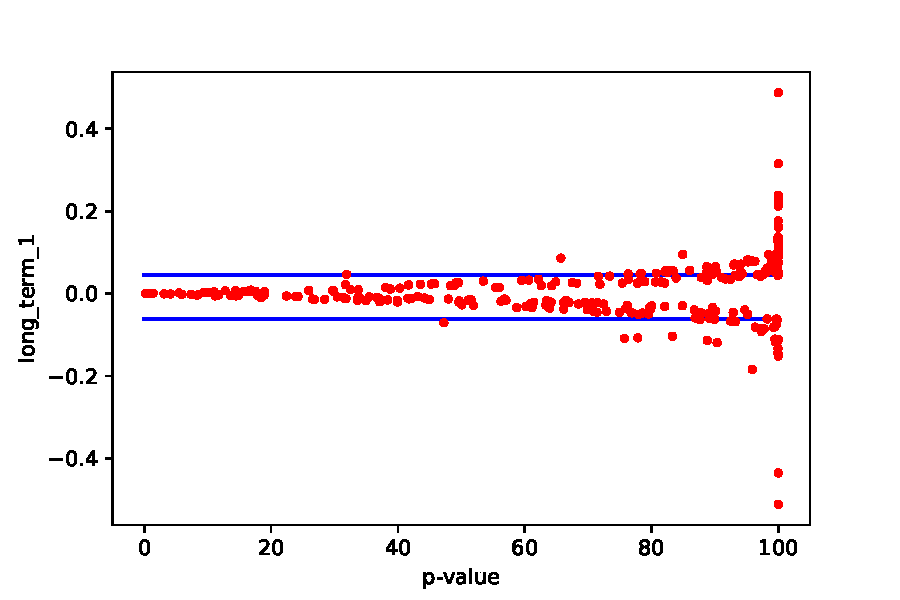
\includegraphics[scale=1]{thresholds.pdf}
		\caption{Распределение отклонений метрики от $p_{value}$}
		\label{fig:metric1}
	\end{figure}
	
	На рисунке \ref{fig:metric1} показано, как стоит интерпретировать значения метрики. Синие линии проведены по наиболее близким к 0 значениям метрики при $p_{value} > 99$. Точки между линиями означают, что метрика не прокрасилась. Выше -- значение увеличилось, ниже -- уменьшилось. Таким образом, задачу можно переформулировать как задачу иерархической бинарной классификации: изменилась ли метрика и если да, то как? \\
	
	Первая статья рассказывает о способе создания прокси-метрики, которая была бы чувствительнее (имела бы больший z-score), чем используемые метрики. В условиях текущей задачи хотелось бы создать такую прокси-метрику из short-term метрик и оценить, насколько её изменение влечёт изменение таргет-метрики (одной из long-term метрик).
	К сожалению, данных для оптимизации функции потерь из исследования нет, так как она требует матрицы вариаций всех признаков. Поэтому была рассмотрена упрощённая целевая функция:
	
	$$J(w) = \frac{1}{\|\mathbb{E}\|}\sum_{e\in \mathbb{E}}X_e^T wy_e - \frac{\alpha}{\|\mathbb{C}\|}\sum_{c\in \mathbb{C}}|X_c^T w| %\frac{\beta}{\|\mathbb{U}\|}\sum_{u\in \mathbb{U}}|X_u^T w| 
	$$
	
	Здесь $E$ --- множество экспериментов, в которых таргет-метрика treatment и control группы отличается, то есть $p_{value} > 99$ для этой метрики. $C$ --- множество $A/A$-экспериментов. В текущем датасете таких экспериментов в явном виде нет, поэтому такими экспериментами считаются те, у которых $p_{value} < threshold$ для текущего таргета (здесь стоит заметить, что это тоже неправильно, справедливо такими считать эксперименты, у которых все или хотя бы "почти все" $p_{value} <threshold $).
	
	Смысл такой функции следующий: хочется, чтобы первое слагаемое было большим по модулю и нужного знака (так как произошло изменение), а второе должно иметь маленький модуль, так как изменений не было. Максимизируя эту функцию, можно получить вектор весов, которые будут по short-term метрикам предсказывать один из трёх классов для long-term метрики: $+1, 0, -1$. \\

	Этот метод стоит исследовать более внимательно, на данный момент есть следующие трудности, по сравнению со вторым методом:
	\begin{enumerate}
		\item Более сложная для интерпретации метрика.
		\item Гиперпараметр для threshold у АА-тестов (этой проблемы не будет, когда будут данные АА-тестов). Чем этот трешхолд выше, тем больше экспериментов считается АА-тестированием, тем выше вес второго слагаемого целевой функции.
		\item Гиперпараметр $\alpha$, являющийся явным весом второго слагаемого.
		\item Неустойчивость решения в зависимости от начальных условий даже при одинаковых гиперпараметрах (зависит от начального приближения).
	\end{enumerate}
		
	Вторая статья предлагает решать задачу регрессии вместо задачи классификации. Решением будет умножение вектор весов как: $w = X^+y$, где $X$ --- матрица, где $x_{ij}$ --- значение short-term метрики $j$ в эксперименте $i$, $y$ --- вектор значений long-term метрики, а $X^+$ --- псевдообратная матрица $X$. Однако в таком случае будут учтены изменения с низким $p_{value}$. Поэтому даже если $MSE$ уменьшится, вектор весов будет учитывать изменения, не имеющие статистического значения. Поэтому перед вычислением весов делается $l_0$ регуляризация, то есть $X$ преобразуется в вектор $X^q$, где 
	
	\begin{equation*}
		X^q_{ij} = 
		\begin{cases}
			0 &\text{$pvalue_{ij} < 99$}\\
			X_{ij} &\text{иначе}
		\end{cases}
	\end{equation*}
	И уже после этого находится вектор весов как 
	
	$$w = (X^q)^+y$$
	
	Результат: $MSE \approx 0.75$. Эту величину можно уменьшать, ориентируясь на меньшее количество экспериментов (исключая "выбросы" с помощью OneClassSVM на short-term метрики). Однако заметные изменения происходят уже при $\nu \approx 0.4$, таким образом теряется существенная часть данных (тестирование тоже происходит на "чистых" данных). На рисунке \ref{fig:mse} показана соответствующая зависимость. \\
	
	\begin{figure}[h]
		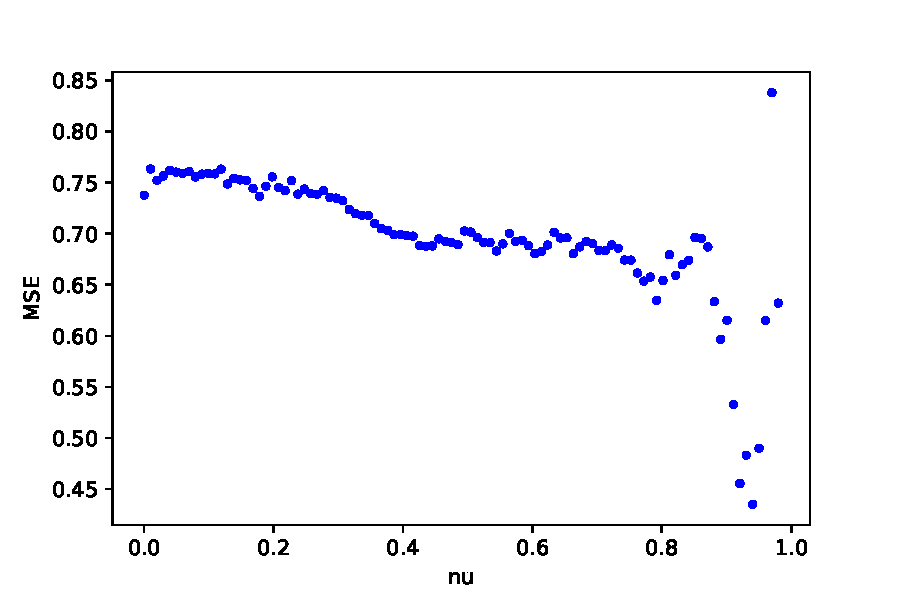
\includegraphics[scale=1]{MSE_nu_dependency.pdf}
		\caption{Зависимость MSE от $\nu$ (доли "выбросов")}
		\label{fig:mse}
	\end{figure}
	
	Хочется наблюдать за устойчивостью вектора весов при разных наборах коротких метрик в данных. То есть существует гипотеза о том, что вес короткой метрики, хорошо коррелирующей c измеряемой таргет-метрикой, не должен сильно измениться при изменении множества обучаемых атрибутов. Как минимум у устойчивой короткой метрики не должен изменяться знак: нехорошо, если в половине разбиений метрика увеличивает таргет, а в другой половине уменьшает. Иллюстрация этого приведена на рисунке \ref{fig:weight_dispersion}.
	
	\begin{figure}[htp]
		
		\centering
		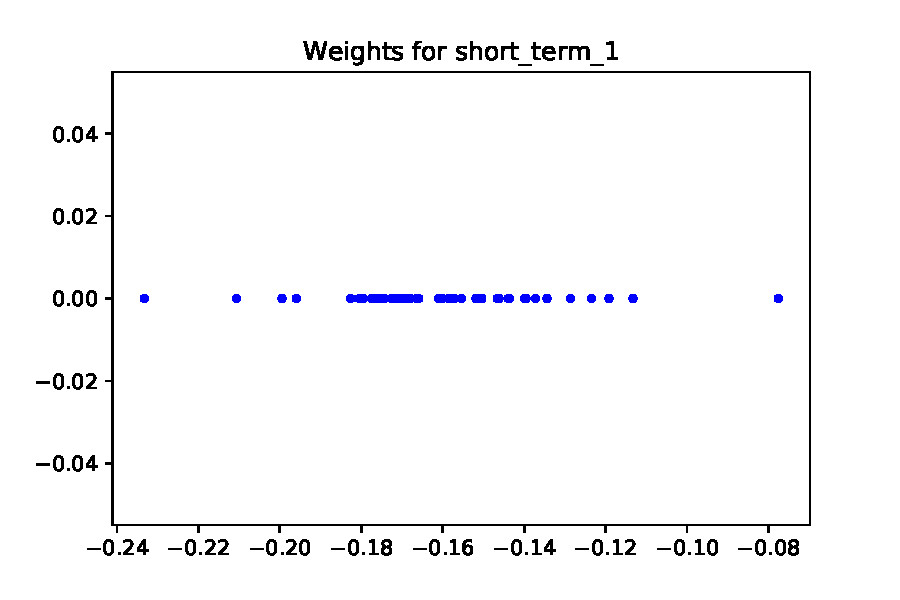
\includegraphics[width=.6\textwidth]{weights_short_term_1.pdf}\hfill
		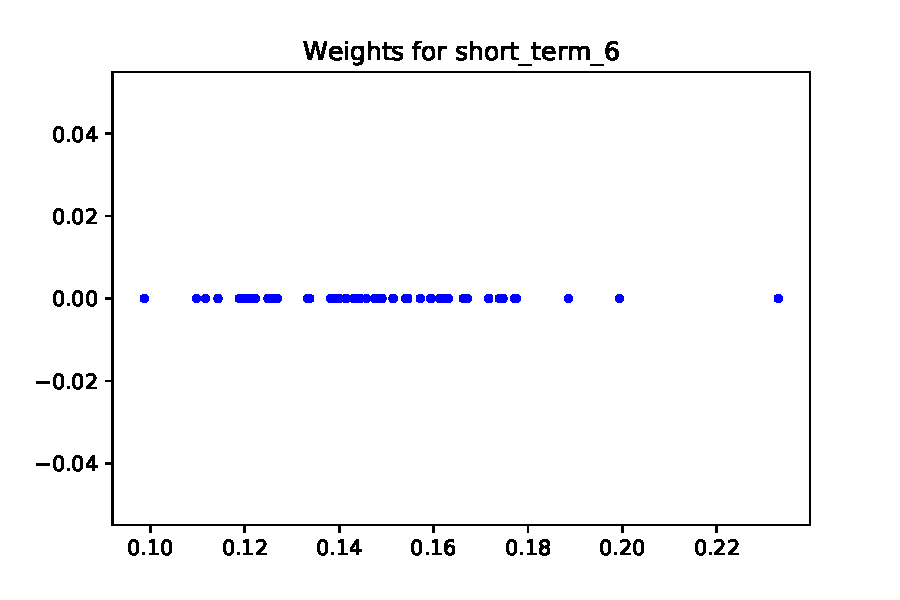
\includegraphics[width=.6\textwidth]{weights_short_term_6.pdf}\hfill
		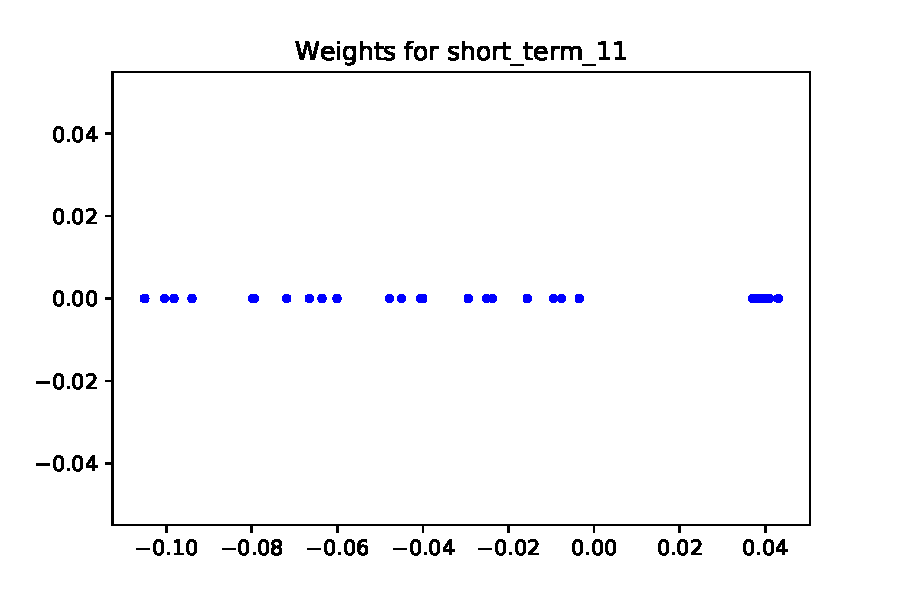
\includegraphics[width=.6\textwidth]{weights_short_term_11.pdf}
		
		\caption{Веса коротких метрик в моделях, обученных на разных подмножествах метрик. Первые два графика показывают "хорошую" метрику. То есть знак для них всегда оставался фикисированным на разных разбиениях. В то время, как последняя метрика даёт вес разного знака в зависимости от подмножества обучаемых метрик и хорошей не является.}
		\label{fig:weight_dispersion}
	\end{figure}



	
\end{document}